\documentclass[conference,onecolumn]{IEEEtran}
\usepackage{hyperref}
\usepackage[utf8]{inputenc}
\usepackage[french]{babel}
\usepackage{amsmath,amssymb,amsfonts}
\usepackage{algorithmic}
\usepackage{graphicx}
\usepackage{textcomp}
\usepackage{xcolor}
\usepackage{lipsum, babel}
\def\BibTeX{{\rm B\kern-.05em{\sc i\kern-.025em b}\kern-.08em
    T\kern-.1667em\lower.7ex\hbox{E}\kern-.125emX}}
\begin{document}

\title{Atténuation du bruit dans des signaux audios a travers l’implémentation de méthodes classiques et une méthode hybride\\
}

\author{\IEEEauthorblockN{1\textsuperscript{st} José Miguel Galindo Barco}
\IEEEauthorblockA{\textit{Ecole d’ingénieurs}\\
\textit{Génie de systèmes} \\
\textit{Université EAFIT}\\
\href{mailto:jmgalindob@eafit.edu.co}{jmgalindob@eafit.edu.co}
}
\and
\IEEEauthorblockN{2\textsuperscript{nd} Juan José Tamayo Acevedo}
\IEEEauthorblockA{\textit{Ecole de sciences}\\
\textit{Génie mathématique} \\
\textit{Université EAFIT}\\
\href{mailto:jjtamayoa@eafit.edu.co}{jjtamayoa@eafit.edu.co}
}
\and
\IEEEauthorblockN{3\textsuperscript{rd} Salomón Cardeño Luján}
\IEEEauthorblockA{\textit{Ecole de sciences}\\
\textit{Génie mathématique} \\
\textit{Université EAFIT}\\
\href{mailto:scardenol@eafit.edu.co}{scardenol@eafit.edu.co}
}
}

\maketitle

\begin{abstract}
L’atténuation du bruit est un domaine d’étude actif dans des milieux comme le traitement digital et analogique des signaux. Dans ce domaine il existe une grande variété d’algorithmes et/ou méthodes classiques et modernes qui sont utilisé dans ce but. Dans ce travail de recherche, nous réaliserons une étude théorique du filtre analogique passe-bas avec une approximation de Butterworth, le filtre de Weiner et la méthode dite hybride de DSP/Deep Learning RNNbruit. Puis nous développerons une analyse de ces trois méthodes où nous comparerons les résultats de signaux lorsque nous filtrons un signal propre, un signal avec addition de bruit blanc, un signal avec addition de bruit rosa et un signal avec addition de bruit rouge. Les enregistrement audios résultant de chaque méthode filtrage seront comparer qualitativement et quantitativement, d’où la nécessité de tenir en compte la perception auditive du récepteur. Finalement, nous proposerons des modifications sur la mise en œuvre ou implémentation de ces méthodes en considérant le contexte et le bon fonctionnement dans ce dernier. 
\end{abstract}

\section{Introduction}
%\lipsum[1]

\section{Concepts fondamentaux}

Signal: un signal est la representation physique de l'information, qu'il convoit de sa source a sa destination.


Bruit: Un bruit correspond a tout phénomène gênant la transmission ou l'interpretation d'un signal

Traitement du signal : Le traitement du signal est une discipline qui étudie des méthodes de traitement, d’analyse et d’interprétation des signaux. Pour cela, dans ce domaine on utilise des méthodes tels que le contrôle, le filtrage, la compression et la transmission de données, la réduction du bruit, la déconvolution, la prédiction, l'identification, la classification.  


Filtrage : On appelle "filtrage" toute application qui, à un signal fe(t), dit "signal d'entrée", associe un signal fs(t), dit "signal de sortie", tel que le module du spectre de fs(t) soit inférieur ou égal au module du spectre de fs(t), pour w réel quelconque. 

\subsection{Signal sonore et note audio}
Le son ou signal sonore est une perturbation mécanique d’un état d’équilibre, qui se propage à travers d’un milieu solide élastique. Il est possible de le définir subjectivement comme ceux qui est perçu par l’ouïe, mais cela reviendra à restreindre la définition même d’un signal. De même, la lumière est perçue par la vue mais il existe certaines longueurs d’ondes lumineuse qui ne sont pas perçu par l’œil humain. Il existe donc des domaines de fréquences des signaux sonores qui ne sont pas perçu par l’ouïe humain. 

Dans un premier temps, en s’appuyant sur le point de vue physique, les ondes sonores se propage à travers l’air ou autres milieux (solides et élastiques) sous forme de longueur d’ondes, où la vibration mécanique qui décrit l’onde se propage dans la même direction que la propagation de celle-ci. L’air peut être compris comme un milieu élastique sur lequel les particules, ou tout simplement les couches d’air, ont un comportement semblable à un ressort, c’est-à-dire qu’elles “se poussent” et “s’attirent” les unes avec les autres. 

\subsection{Caractéristiques physique et description mathématique d’un signal sonore }

Il est important de remarque que dans figure précédente, plus précisément dans la partie C de cette figure, s’agit d’une autre représentation du signal sonore illustré dans la partie B. En effet, dans cette partie nous pouvons voire une courbe sinusoïdale, cette courbe représente la variation de la pression du signal sonore, celui-ci se répète de façon périodique. La distance entre 2 pics de la courbe est nommée longueur d’onde et se représente par la lettre λ. 

Lorsqu’un signal sonore ou onde sonore se déplace dans l’air, la longueur d’onde prend un certain temps pour aller d’un point A à un point B de l’espace, cette durée de temps est appelée période et note T. 

De plus, pendant un intervalle de temps équivalent à une seconde, un certain nombre de longueurs d’onde passe d’un point A à un point de l’espace. Ce phénomène est connu comme fréquence du signal. Dans d’autres mots, la fréquence est le nombre de périodes par unité de temps ce qui correspond à l’inverse de la période : f=1/T ou f est la fréquence en Hertz (Hz ou s-1) et T la période en seconde (s). 



Il est important de remarquer que les signaux sonores qui ont de hautes fréquences, ont des périodes courtes, alors que les signaux sonores qui ont des bases fréquences, ont de longs périodes. De plus, l’intervalle de fréquences que l’être humain peut percevoir se trouve entre les 20Hz et les 20 kHz. Il existe une propriété physique qui permet de classifier les signaux sonores en fonction de la perception physiologique des êtres humains, cette propriété est connue comme le ton. En plus, les signaux ont une vitesse de déplacement, celle-ci est connue comme vitesse de l’onde (S), elle est obtenue par une relation entre la fréquence ou la période et la longueur d’onde, comme montrer ci-dessous : 

 S = f*λ = λ/T

Le déplacement d’une onde sonore dans une dimension (signal sonore plat) est décrit mathématiquement par l’équation général du mouvement des ondes, qui peut être écrit de la façon suivante :  

 
y(x,t) = A*sin(2*π*(f*t - x/λ)
 

L'amplitude (A)d'une onde correspond à la hauteur maximale atteinte par l'onde par rapport à sa position n au repos. 

De plus, grâce à l’amplitude nous pouvons déterminer intensité de l’onde, qui est perçu par l’ouïe sous le nom de volume. L'intensité acoustique (I), est définie comme le taux de transmission d'énergie par unité d’aire perpendiculaire à la direction de propagation de l’onde. La relation existante entre l’intensité et l’amplitude est la suivante : 

 I = A*A/2*ρ*S

Avec :  

- ρ : densité de l’air à l’équilibre (en kg/m³). 

 - S vitesse de l’onde (en m/s) 

L’intensité I a pour unité les watt par mètre carré (W/m²). Sous des “conditions atmosphériques standards, on a : 

 

L’amplitude minimum de variation de pression que l’ouïe humain peut percevoir es de 10-5 Pa et l’amplitude maximal est de 10 Pa. 

\subsection{Audition et perception du son chez les êtres humains}

D’après ce qui a été décrit précédemment, il est convenable de remarque les faits suivants : 

- Entre 20 Hz et 20 kHz se trouve l’intervalle de fréquence perçu par l’être humain.  

- L’amplitude d’une onde sonore permet de déterminer l’intensité de l’onde. 

- L’amplitude minimum de variation de pression que l’ouïe humain peut percevoir es de 10-5 Pa et l’amplitude maximal est de 10 Pa. 

Echelles des décibels 

L’échelle des décibels est une échelle qui permet de classifie les ondes sonores en fonction de leur intensité sonore. Cette échelle est décrite par l’équation suivante : 

I = L = 10*log(I/I0) 

Avec L qui représente les décibels, I l’intensité de l’onde et I0 es l’intensité de référence. 

Plus précisément, L’échelle des décibels est logarithmique, ce qui signifie qu’une augmentation du niveau sonore de 3 dB représente déjà un doublement de l’intensité sonore. Par exemple, le volume d’une conversation normale peut être d’environ 65 dB et, pour quelqu’un qui crie, ce chiffre peut atteindre environ 80 dB. La différence est seulement de 15 dB, mais le cri représente une intensité trente fois supérieure. 

Le décibel (dB) est une unité utilisée pour mesurer l'intensité des sons et celle d'autres grandeurs physiques. Un décibel équivaut à un dixième de bel (B), une unité qui doit son nom à Graham Bell, l'inventeur du téléphone. Son échelle logarithmique permet de représenter le spectre auditif de l’être humain dans son ensemble. 

 Le champ auditif de l’être humain (en vert) est limité par une courbe qui nous fournis la limite inferieur et une autre courbe qui nous donne la limite supérieure de la perception sonore. A caque fréquence, entre 20 Hz et 20 kHz, le seuil de notre sensibilité est différent. L’intervalle le plus large de perception a lieu aux alentours les 2 kHz et commence à partir des 0 dB. Dans cet intervalle dit “moyen” les dynamiques sensorielles sont les plus aptes possibles et peuvent avoir un équivalent de 130 dB.  
 
 \subsection{Tonalité pure}
 Lorsque nous utilisant de fonction comme celle de la vitesse de déplacement d’une onde, nous pouvons dire que cette fonction représente une tonalité pure avec un fréquence f. Ce nom dérive du fait que cette fonction décrit une onde sonore avec une seule composante en fréquence, c’est-à-dire qu’il s’agit d’un cas idéal, parce que en faisant analogie avec la lumière, dans la nature nous ne trouverons jamais une lumière monochromatique (d’une seule couleur, c’est-à-dire d’une seule fréquence), nous ne trouverons jamais une onde sonore avec cette caractéristique.  

Afin de donner une définition plus précise d’une tonalité pure, nous devons nous appuyer sur la définition donnée en psychoacoustique. En effet, en psychoacoustique, une tonalité pure, ou encore son pur ou note pure (en anglais : pure tone) est un son avec une forme d'onde sinusoïdale ; c'est-à-dire une onde sinusoïdale de n'importe quelle fréquence, phase et amplitude1. En audiologie clinique, les tons purs sont utilisés pour l'audiométrie tonale (en) afin de caractériser les seuils d'audition à différentes fréquences. 

\subsection{Decomposition spectral ou echantillonage}

L'échantillonnage d'un signal continu est l'opération qui consiste à prélever des échantillons du signal pour obtenir un signal discret, c'est-à-dire une suite de nombres représentant le signal, dans le but de mémoriser, transmettre, ou traiter le signal. 

L'échantillonnage intervient dans l'opération de conversion analogique-numérique, par exemple dans un dispositif de numérisation du son ou de l'image. Un autre exemple d'échantillonnage est celui que l'on fait pour obtenir la représentation graphique d'une fonction à une ou deux variables. D'une manière générale, l'échantillonnage intervient dans toute opération de conversion continu/discret. 

Le théorème de l'échantillonnage de Shannon, qui permet de savoir à quelle fréquence minimale il faut échantillonner un signal pour ne pas perdre l'information qu'il contient. 

Soit u(t) une fonction représentant un signal continu. On considère un échantillonnage périodique défini par : 

 

où k est un entier. Te est la période d'échantillonnage. fe=1/Te est la fréquence d'échantillonnage. 

Le théorème de Shannon ([1]) concerne les signaux dont le spectre possède une fréquence maximale fmax, que l'on appelle des signaux à bande limitée. Par exemple, si u(t) est un polynôme trigonométrique, la fréquence maximale est celle de la plus grande harmonique. 

Théorème de Shannon : pour que le signal puisse être entièrement reconstruit à partir des échantillons, il faut et il suffit que : 

 

La fréquence d'échantillonnage doit être strictement supérieure à deux fois la plus grande fréquence présente dans le spectre du signal continu (condition de Nyquist-Shannon). Si cette condition est vérifiée alors : 

 

où la fonction sinus cardinale est définie par : 

 

Cette relation montre que le signal peut être reconstruit à partir des échantillons, ce qui signifie que toute l'information présente dans le signal original est conservée dans les échantillons. Nous verrons plus loin comment l'opération de reconstruction est effectuée en pratique. 

La moitié de la fréquence d'échantillonnage est appelée la fréquence de Nyquist fn et la condition de Nyquist-Shannon s'écrit donc fmax<fn. 

Lorsque la condition n'est pas vérifiée, on dit qu'il y a sous-échantillonnage. On parle de sur-échantillonnage lorsque la fréquence de Nyquist est beaucoup plus grande que fmax. 


\subsection{Représentation d’un fichier audio dans un ordinateur}
%\lipsum[3]

\subsection{Bruit et types de bruit}
Comme vue précédemment, le bruit dans un signal sonore correspond à une perturbation de celui-ci entrainant des pertes de d’information. Il existe plusieurs types de bruit qui ont leurs propres domaines de fréquences et qui altèrent ou modifient l’information contenue dans un signal de façon différente. En effet, entre les différents types de bruits nous pouvons remarqués 2 groupes très importants : Les bruits dit naturels et les bruits dit industriels.  

Dans un premier temps, en regardant les bruits naturels nous pouvons nous rendre compte que ces bruits ne sont pas produits de façon artificielle et existe par différentes raisons. Dans cette famille de bruit nous pouvons trouvés le bruit ambiant qui correspond au bruit total existant dans une situation donnée pendant un intervalle de temps donné, ainsi que les bruits qui le compose telles que le bruit résiduel et le bruit particulier. De plus, nous trouvons aussi des bruits dis colorées telles que le bruit blanc ou le bruit rose, qui feront objet de notre étude de filtrage. Tout d’abord, il faut remarquer que le bruit blanc est un bruit composé par la somme de tous le bruit coloré, c’est à dire l’addition en fréquence du bruit rose, bruit rouge ou brownien, bruit bleu ou azur, bruit violet et bruit gris. Chacun d’entre eux aillant un domaine de fréquence particulier et des caractéristique propre. Par exemple : 

 - Le bruit rouge ou brownien correspond dans une première approximation, dans les domaines qui utilisent des définitions précises, la terminologie « bruit rouge », « bruit brownien » ou « bruit brun » fait référence au son ayant une puissance sonore qui décroît de 6 dB par octave lorsque la fréquence augmente (densité proportionnelle à 1/f ) sur un intervalle de fréquence n'incluant pas de DC (Qui dans un sens général, n'inclut pas de composante constante, ou de valeur pour f=0). 

D’un autre point de vue, dans les domaines qui utilisent des définitions plus approximatives, le « bruit rouge » correspond à tout son dont la densité de puissance diminue lorsque la fréquence augmente3. 

Plus exactement Le bruit rouge, peut être obtenu en utilisant un algorithme simulant le mouvement brownien ou par intégration mathématique du bruit blanc.  

- Le bruit bleu qui correspond à un bruit qui augmente sa puissance sonore de 3 dB par octave lorsque la fréquence augmente (densité proportionnelle à f), et ce jusqu’à une fréquence infinie. 

Dans le domaine de l’informatique graphique, le terme « bruit bleu » est parfois utilisé d’une façon plus approximative pour décrire tout son de puissance sonore minimale à basse fréquence et ne présentant aucun pic lorsque la fréquence augmente (croissance constante). 

Il est convenable de connaitre et différencier aussi le bruit rose des autres types de bruits coloré, dans la mesure que ce type de bruit fait partie de notre étude. Donc le bruit rose, ce type de bruit est caractérisé par une puissance égale sur des bandes proportionnelles en largeur. Une bande correspond en fait à un changement de fréquence (hausse ou baisse à exprimer en pourcentage de l’une des extrémités de l’intervalle). Par exemple, la puissance d’un bruit rose est la même sur les intervalles allant de 40 à 60 Hz et de 4 000 à 6 000 Hz car ces intervalles sont proportionnels (ils correspondent à une hausse de 50 pourcent de la fréquence). 

Dans un deuxième temps, nous voyons l’existence d’une deuxième famille de bruits que nous choisissant de nommé des bruits industriels. En effet, comme son nom l’indique les bruits industriels sont des perturbations sonores produits par l’industrie ou par des effet industrie. Dans cette famille nous trouvons des bruits tels que le bruit de route qui est un bruit normalisé. Il est une référence pour le bruit des trafics routiers et ferroviaires. Son spectre est enrichi en basses fréquences et appauvri dans les aiguës par rapport à un bruit rose. Mais aussi nous trouvons des bruits comme les suivants : 

Le bruit d’impact : c’est le bruit transmis par une paroi mise en vibration par un choc (bruit de pas, déplacement de meubles, chute d’objet, enfoncement d’un clou dans un mur...). 

 Le bruit aérien : c’est le bruit propagé dans l’air (bruit de voix, bruit de télévision, bruit de circulation...). 

Le bruit solidien : c’est le bruit propagé dans les milieux solides comprenant (le bruit d’impact transmis par les éléments solides, le bruit d’équipement (chaufferie, ascenseurs, ...). 

\section{Méthodes}
Le but de ce projet est de implementer le filtrage dans les notes audios dans l'objectif d'attenuer le bruit present. Pour cela nous allons implementé le filtrage analogique avec une approximation de Butterworth, la méthode RNN et un autre qui reste définir.

\section{Résultats et comparaison des méthodes}

\begin{figure}[htp]
    \centering
    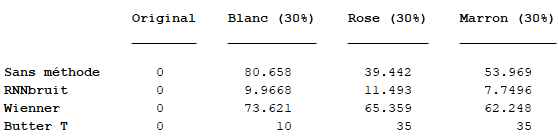
\includegraphics[width=15cm]{Tabla.png}
    \caption{Résultats des méthodes pour 30\% du bruit blanc, rose et marron.}
    \label{fig:Résultats}
\end{figure}

Premièrement, en étudiant les résultats obtenus par l'implémentation du filtre passe-bas avec une approximation de Butter Worth, nous confirmant les hypothèses théoriques vues précédemment. En effet, compte tenu que l’approximation de Butter Worth permet d’avoir une précision en amplitude. Cette précision est centre sur des bases fréquences. Nous voyons cela évidence dans le filtrage des bruits ajouter à notre signal. Lorsque nous ajoutons du bruit blanc et nous filtrons le signal résultant, nous constatons une diminution du pourcentage du bruit présent dans le signal. Alors que lorsque nous effectuons le même procédé pour le bruit rose et le bruit marron, le pourcentage de bruit ne change pas. Donc cette méthode avec cette approximation particulière est bien plus convenable pour filtrer le bruit blanc présent dans les enregistrements audios.

Dans un deuxième temps, le cas de la méthode hybride du RNNbruit, nous observons que cette méthode est belle et bien convenable pour les différents types de bruit additionnés. En effet, nous constatons une atténuation du bruit considérable dans chacun des cas. De plus, nous remarquons que cette méthode ne gêne pas la transmission du signal sonore, en d'autre thermes cette méthode lise et "purifie" le signal orignal. Nous pouvons expliquer ce comportement par la nature adaptative de la méthode, dû au fait de l'implémentation de réseau de neurones récurrents pour faire face au bruit non harmonique. Cependant, la partie traditionnelle de cette méthode dite hybride se charge du bruit harmonique comme nous l'avant vue précédemment dans la partie théorique.

Finalement, lorsque nous analysons les résultats obtenus en utilisant le filtre adaptatif de Weiner, nous apercevons que cette méthode de filtrage numérique a des meilleurs résultats sur du bruit blanc. Or, en effectuant une analyse auditive, nous pourrions penser que ce filtrage est bien plus efficace avec le bruit marron ou le bruit rose, nous pouvions affirmer théoriquement que ‘est avec le bruit blanc qu’il est plus efficace. En effet, en employant cette méthode nous introduisons des nouveaux types de bruits que nous ne considérerons pas dans notre analyse. Par exemple, dans le filtrage de l’enregistrement audio avec du bruit marron, nous pouvons avoir l’impression que le résultat est nettement plus compressible qu’avec du bruit blanc. Cependant, en regardant les résultats de l’analyse nous nous rends compte que l’audio résultant a perdu de l’intensité sonores, c’est-à-dire que l’amplitude de son gain en fréquence a considérablement diminuer. Cette méthode, théoriquement parlant, nous est convenable dans la mesure ou elle permet un filtrage du bruit blanc, mais elle rencontre ses limites avec les 2 autres types de bruit étudiés.


\end{document}